%; whizzy paragraph -pdf xpdf -latex ./whizzypdfptex.sh
%; whizzy-paragraph "^\\\\begin{frame}\\|\\\\emtext"
% latex beamer presentation.
% platex, latex-beamer $B$G%3%s%Q%$%k$9$k$3$H$rA[Dj!#(B 

%     Tokyo Debian Meeting resources
%     Copyright (C) 2012 Junichi Uekawa

%     This program is free software; you can redistribute it and/or modify
%     it under the terms of the GNU General Public License as published by
%     the Free Software Foundation; either version 2 of the License, or
%     (at your option) any later version.

%     This program is distributed in the hope that it will be useful,
%     but WITHOUT ANY WARRANTY; without even the implied warreanty of
%     MERCHANTABILITY or FITNESS FOR A PARTICULAR PURPOSE.  See the
%     GNU General Public License for more details.
%     You should have received a copy of the GNU General Public License
%     along with this program; if not, write to the Free Software
%     Foundation, Inc., 51 Franklin St, Fifth Floor, Boston, MA  02110-1301 USA

\documentclass[cjk,dvipdfmx,12pt]{beamer}
\usetheme{Tokyo}
\usepackage{monthlypresentation}

%  preview (shell-command (concat "evince " (replace-regexp-in-string "tex$" "pdf"(buffer-file-name)) "&")) 
%  presentation (shell-command (concat "xpdf -fullscreen " (replace-regexp-in-string "tex$" "pdf"(buffer-file-name)) "&"))
%  presentation (shell-command (concat "evince " (replace-regexp-in-string "tex$" "pdf"(buffer-file-name)) "&"))

%http://www.naney.org/diki/dk/hyperref.html
%$BF|K\8l(BEUC$B7O4D6-$N;~(B
\AtBeginDvi{\special{pdf:tounicode EUC-UCS2}}
%$B%7%U%H(BJIS$B7O4D6-$N;~(B
%\AtBeginDvi{\special{pdf:tounicode 90ms-RKSJ-UCS2}}

\newenvironment{commandlinesmall}%
{\VerbatimEnvironment
  \begin{Sbox}\begin{minipage}{1.0\hsize}\begin{fontsize}{8}{8} \begin{BVerbatim}}%
{\end{BVerbatim}\end{fontsize}\end{minipage}\end{Sbox}
  \setlength{\fboxsep}{8pt}
% start on a new paragraph

\vspace{6pt}% skip before
\fcolorbox{dancerdarkblue}{dancerlightblue}{\TheSbox}

\vspace{6pt}% skip after
}
%end of commandlinesmall

\title{$BEl5~%(%j%"(BDebian$BJY6/2q(B}
\subtitle{$BBh(B136$B2s(B 2016$BG/(B2$B7nEY(B}
\author{$BLnEg5.1Q(B}
\date{2016$BG/(B2$B7n(B13$BF|(B}
\logo{
\includegraphics[width=8cm]{image200607/openlogo-light.eps}}

\begin{document}

\begin{frame}
\titlepage{}
\end{frame}

\begin{frame}{Agenda}
 \begin{minipage}[t]{0.45\hsize}
  \begin{itemize}
   \item $B;vA02]BjH/I=(B
   \item $B:G6a$"$C$?(BDebian$B4XO"$N%$%Y%s%HJs9p(B
	 \begin{itemize}
	 \item $BBh(B135$B2sEl5~%(%j%"(BDebian$BJY6/2q(B
	 \end{itemize}
  \end{itemize}
 \end{minipage} 
 \begin{minipage}[t]{0.45\hsize}
  \begin{itemize}
   \item Debian Trivia Quiz
   \item Debian GNU/Linux $B>e$G$N>JEENO@_Dj$K$D$$$F(B
   \item libhinawa $B$H$$$&%i%$%V%i%j$r(B Debian $B%W%m%8%'%/%H$K(B ITP/RFS $B$7$?OC(B
   \item $B:#F|$N1c2q>l=j(B
  \end{itemize}
 \end{minipage}
\end{frame}

\section{$B;vA02]Bj(B}
\emtext{$B;vA02]Bj(B}
{\footnotesize
 \begin{prework}{ takaswie }
  \begin{enumerate}
  \item Q.hack time に何をしますか?\\
    A.hinawa-utils の開発。あるいはALSAの開発。\\
https://github.com/takaswie/hinawa-utils
  \item Q.本勉強会をどこでお知りになりましたか?(任意回答)\\
    A. ML
  \end{enumerate}
\end{prework}


\begin{prework}{ mkouhei }
  \begin{enumerate}
  \item Q.hack time に何をしますか?\\
    A.
    \begin{itemize}
    \item https://qa.debian.org/developer.php? login=mkouhei@palmtb.net のメンテ。
    \item パッケージ ( https://qa.debian.org/developer.php? login=mkouhei@palmtb.net ) のメンテナンス
    \item keybase.io を signing-party( caff ) のキーサーバーとして利用できないかの検証

   \end{itemize}
    \item Q.本勉強会をどこでお知りになりましたか?(任意回答)\\
    A. 常連
   \end{enumerate}
\end{prework}

\begin{prework}{ Poeto }
  \begin{enumerate}
  \item Q.hack time に何をしますか?\\
    A.「 Debian 」 の基本操作。( 数日前、インストールしたばかりなので )
  \item Q.本勉強会をどこでお知りになりましたか?(任意回答)\\
    A. Web
  \end{enumerate}
\end{prework}

\begin{prework}{ kenhys }
  \begin{enumerate}
  \item Q.hack time に何をしますか?\\
    A. 未定。
  \item Q.本勉強会をどこでお知りになりましたか?(任意回答)\\
    A. ML
  \end{enumerate}
\end{prework}

\begin{prework}{ iwamatsu }
  \begin{enumerate}
  \item Q.hack time に何をしますか?\\
    A. package メンテナンス。
  \item Q.本勉強会をどこでお知りになりましたか?(任意回答)\\
    A. ML
  \end{enumerate}
\end{prework}

\begin{prework}{ Charies }
  \begin{enumerate}
  \item Q.hack time に何をしますか?\\
    A. パッケージング。
  \end{enumerate}
\end{prework}

\begin{prework}{ dictoss }
  \begin{enumerate}
  \item Q.hack time に何をしますか?\\
    A. kfreebsd の Intel GPU ビデオドライバのデバッグ( unstable で動かなくなった)
  \item Q.本勉強会をどこでお知りになりましたか?(任意回答)\\
    A. Web
  \end{enumerate}
\end{prework}

\begin{prework}{ rosh }
  \begin{enumerate}
  \item Q.hack time に何をしますか?\\
    A. d-i に関する作業
  \item Q.本勉強会をどこでお知りになりましたか?(任意回答)\\
    A. twitter
  \end{enumerate}
\end{prework}

\begin{prework}{ wskoka }
  \begin{enumerate}
  \item Q.hack time に何をしますか?\\
    A. tilegx
  \end{enumerate}
\end{prework}

\begin{prework}{ yy\_y\_ja\_jp }
  \begin{enumerate}
  \item Q.hack time に何をしますか?\\
    A. DDTSS
  \end{enumerate}
\end{prework}

\begin{prework}{ 野島 }
  \begin{enumerate}
  \item Q.hack time に何をしますか?\\
    A. DDTSS、xmrisパッケージ化など。
  \item Q.本勉強会をどこでお知りになりましたか?(任意回答)\\
    A. 幹事なので!\\ところでセミナか、幹事やってみたい人はいつでも募集中!\\貴殿好みの勉強会にしてくれてもよくてよ!
  \end{enumerate}
\end{prework}


}

\section{$B%$%Y%s%HJs9p(B}
\emtext{$B%$%Y%s%HJs9p(B}

\begin{frame}{$BBh(B135$B2sEl5~%(%j%"(BDebian$BJY6/2q(B }

\begin{itemize}
\item $B>l=j$O(Bdots$B$5$s$r$*<Z$j$7$F$N3+:E$G$7$?!#(B
\item $B;22C<T$O(B10$BL>$G$7$?!#(B
\item $B%;%_%JFbMF$O!"(B2$BK\7z$F$G!"(B
  \begin{enumerate}
  \item $B;22C<T3'$5$s$K$h$k!V(B Debian $B:#G/$NH>G/J,$N7W2h$rN)$F$F$_$?(B $B!W(B
  \item $BLnEg$5$s$K$h$k!V(B Debian $B$G(B Linux Ftrace $B$^$o$j$r$$$8$C$F$_$?(B  $B!W(B
  \end{enumerate}
$B$G$7$?!#(B
\item $B;D$j$N;~4V$G(Bhack time$B$r9T$$!"@.2LH/I=$r$7$^$7$?!#(B
\end{itemize} 
\end{frame}

\begin{frame}{$BBh(B135$B2sEl5~%(%j%"(BDebian$BJY6/2q(B($B$D$E$-(B)}

  $B!V(BDebian $B:#G/$NH>G/J,$N7W2h$rN)$F$F$_$?!W$O!"(B2016$BG/(B6$B7nKv$^$G$N(BDebian$B%W%m%8%'%/%H$G9T$&L\I8$r=q$$$FD:$-$^$7$?!#$_$J$5$s!"$,$C$A$jL\I8$rN)$F$F$$$?$@$1$^$7$?!#$"$H$O!"<B9T$"$k$N$_$H$$$&$3$H$G!"$h$m$7$/$*$M$,$$$7$^$9!*(B

\end{frame}

\begin{frame}{$BBh(B135$B2sEl5~%(%j%"(BDebian$BJY6/2q(B($B$D$E$-(B)}

  $B!V(BDebian $B$G(B Linux Ftrace $B$^$o$j$r$$$8$C$F$_$?!W$O!"(Blinux kernel$B$KEk:\$5$l$F$$$k%G%P%C%0(BI/F$B$G$"$k(BFtrace$B$r(BDebian$B$GMxMQ$7$F$_$?;v$K$D$$$F8l$i$l$^$7$?!#(BDebian sid$B$KEk:\$5$l$F$$$k(Bkernel$B$,(B4.3.3$B$G$"$k$3$H$+$i!"(BUSDT$B$rMxMQ$7$F$_$?$j!"(Bkprobe$B$rMxMQ$7$?OC$r$7$^$7$?!#(BDebian$B$KEk:\$5$l$F$$$k(BFtrace$BMxMQ$N%D!<%k$G$"$k!"(Bperf-tool$B$,8E$+$C$?7o$K$D$$$F$b!"(BBUG Report\footnote{https://bugs.debian.org/813769}$B$,9T$o$l$^$7$?!#(B

\end{frame}

\begin{frame}{$BBh(B135$B2sEl5~%(%j%"(BDebian$BJY6/2q(B($B$D$E$-(B)}

  Debian$B$O!"%Q%C%1!<%8$,8E$$$J$I$N7o$b(BBUG Report$B$9$k$3$H$G$b2~A1$r?^$k$3$H$,=PMh$^$9!#$b$7!"B>$K!"(B
\begin{itemize}
\item $B%Q%C%1!<%8$,8E$$!"(B
\item $BF3F~$7$?%Q%C%1!<%8$N%=%U%H%&%'%"$N5sF0$,$*$+$7$$!J%P%0$C$F$$$k!K(B
\item $B%Q%C%1!<%8$O$3$&$7$FM_$7$$(B
\end{itemize}
$B$J$I$NMWK>$,$"$j$^$7$?$i!"!VC/$G$b!W(Breportbug$B%D!<%k$r;H$C$F4JC1$K2~A1$NMW@A$r$9$k$3$H$,=PMh$^$9!#@'Hs!"3'MM$b$I$7$I$7(BBUG Report$B$7$F$/$@$5$$$^$;!#(B
  
\end{frame}

\begin{frame}{$BBh(B135$B2sEl5~%(%j%"(BDebian$BJY6/2q(B($B$D$E$-(B)}

  $B$^$?!"(Bhack time$B$G$9$,!"@.2L$r(Btitanpad.com$B$K5-:\$9$k;n$_$r9T$$$^$7$?!#(B
$B0J2<$OA02s$N(Bhack time$BCf$N@.2L$N0lMw$H$J$j$^$9!#(B
\begin{itemize}
\item henrich$B$5$s(B\\
  proposal for Debian idea
  \begin{itemize}
  \item integrate piuparts into repository pipeline
  \item replace dput $\rightarrow$ lintian + piuparts, then upload
   + prevents regression into repository
  \end{itemize}
\item kenhys \\
libhinawa$B$N(Bdebian/*$B$K<j$r$$$l$F$$$/$D$+(BPR$B$rEj$2$?$j!"(Bissue$B$rN)$F$?$j$7$?(B\\
https://github.com/takaswie/libhinawa/pull/20\\
https://github.com/takaswie/libhinawa/pull/21\\
https://github.com/takaswie/libhinawa/pull/24
\end{itemize}
\end{frame}

\begin{frame}{$BBh(B135$B2sEl5~%(%j%"(BDebian$BJY6/2q(B($B$D$E$-(B)}

\begin{itemize}
\item tai$B$5$s(B\\
  \begin{itemize}
  \item $B%-!<%5%$%s$r9T$C$?!#(B caff$B$G$O$J$/<jF0$G(B\\
    Keysigning with the GNU/Linux Terminal\\
    \url{http://www.phillylinux.org/keys/terminal.html}\\
    $B$K1h$C$F$d$C$F$_$?!#$7$+$7:G8e$N=pL>$7$?%-!<$rAw$k=j$,(BGmail$B7PM3$K$J$j=pL>!&0E9f2=$;$:$KJVAw$7$F$7$^$C$?$N$G!"(Bcaff$B$,$d$C$Q$j$$$$$N$+!&!&!&(B
  \item Debian Wiki$B$NK]Lu$7;D$7$NB3$-$r$b$/$b$/$H!#(B
  \end{itemize}
\item wskoka$B$5$s(B\\
  tilegx$BMQ%Q%C%1!<%8:n@.(B(10$B$3$0$i$$!#%H!<%?%k$O#1#2#0#08D$0$i$$$"$k!#!K(B
\end{itemize}
\end{frame}

\begin{frame}{$BBh(B135$B2sEl5~%(%j%"(BDebian$BJY6/2q(B($B$D$E$-(B)}

\begin{itemize}
\item rosh$B$5$s(B\\
  \begin{itemize}
  \item caff $B$G%-!<%5%$%s$,=PMh$?(B\\
  \item $BA0%^!<%8$5$l$?(BLinkstation DTS [0] $B$r%Y!<%9$K$F!"?7(BLinkstation$B%G%P%$%9(B (LS-QVL)$B$N(B DTS $B$rJL$N%f!<%6MM$,=PMh$?$H$NO"Mm$,$"$j$^$7$?!#:#=5<u$1F~$l$i$l$?(B Linkstation DTS [1] $B$K%^!<%8$r9T$$$^$7$?!#$3$l$+$i(B ARM kernel lists $B$K%"%C%W$9$kM=Dj$G$9!#(B\\
    \begin{enumerate}
    \item Kernel tree: arch/arm/boot/dts/kirkwood-{lswvl,lswxl}.dts
    \item \url{http://lists.infradead.org/pipermail/linux-arm-kernel/2016-January/400949.html}
    \end{enumerate}
  \end{itemize}
\end{itemize}
\end{frame}

\begin{frame}{$BBh(B135$B2sEl5~%(%j%"(BDebian$BJY6/2q(B($B$D$E$-(B)}

\begin{itemize}
\item dictoss$B$5$s(B \\
  \begin{itemize}
  \item rasberry pi2$B$N(Bdebian jessie$B$+$i(Bbluetooth$B%F%6%j%s%0$G$-$?(B
  \item $B%-!<%5%$%s$7$^$7$?(B
  \item $BEl5~%(%j%"(BDebian$BJY6/2q$N(Bweb$B%5%$%H$r(BHTML5$BBP1~$H%9%^!<%H%U%)%sBP1~:n6H(B($B%j%]%8%H%j$N>l=j3NG'!"%=!<%9%3!<%I$rFI$s$GCf?H$H:n$j$rGD0.Cf(B)\footnote{2016$BG/(B2$B7n(B27$BF|$KL5;v%j%j!<%9$5$l!"(Btokyodebian.alioth.debian.org$B$O!"=K(B!$B%b%P%$%k%U%l%s%I%j!<$K$J$j$^$7$?(B!}
  \end{itemize}
\item $B#y(B.$B#y$5$s(B
  \begin{itemize}
   \item $B;22C<T$H(Bkey sign$B$r9T$C$?!#(B
   \item Caff$B$G!"N/$^$C$F$$$?(B keysigning $B=hM}$N%-%e!<$r%U%i%C%7%e$G$-$?!#(B
  \end{itemize}
\end{itemize}
\end{frame}

\begin{frame}{$BBh(B135$B2sEl5~%(%j%"(BDebian$BJY6/2q(B($B$D$E$-(B)}

\begin{itemize}
\item takaswie$B$5$s(B\\
$B!!(BEcho Audio Corp.$B$N(BFireworks$B%G%P%$%9%b%8%e!<%k8~$1%3%^%s%I%i%$%s%D!<%k$,$@$$$?$$=q$1$?!#(B\\
\url{https://github.com/takaswie/hinawa-utils}
\item  yy\_y\_ja\_jp$B$5$s(B\\
  \begin{itemize}
  \item uim-qt5 $B%P%0%l%]!<%H(B
  \item $B%-!<%5%$%s(B
  \item DDTSS
  \end{itemize}
\item $BLnEg$5$s(B
  \begin{itemize}
  \item 9$B8D$N(BDDTSS$B$N%l%S%e!<$r9T$$$^$7$?!#$J$*!"(Byorick$B$O(Btypo$B$N(B''M-x Yorick''$B$r8+Mn$H$7!"(Brequeue$B$7$^$7$?!#(B
  \end{itemize}
  
\end{itemize}
\end{frame}

\section{Debian Trivia Quiz}
\emtext{Debian Trivia Quiz}
\begin{frame}{Debian Trivia Quiz}

  Debian $B$N>o<1!"$b$A$m$sCN$C$F$^$9$h$M(B?
$BCN$i$J$$$J$s$FCQ$:$+$7$/$F!"CN$i$J$$$H$O8@$($J$$$"$s$J$3$H$d$3$s$J$3$H!"(B
$B$_$s$J$G3NG'$7$F$_$^$7$g$&!#(B

 $B:#2s$N=PBjHO0O$O(B\url{debian-devel-announce@lists.debian.org},
\url{debian-news@lists.debian.org} $B$KEj9F$5$l$?(B
$BFbMF$J$I$+$i$G$9!#(B

\end{frame}

\subsection{$BLdBj(B}

%; whizzy-master ../debianmeetingresume201311.tex
% $B0J>e$N@_Dj$r$7$F$$$k$?$a!"$3$N%U%!%$%k$G(B M-x whizzytex $B$9$k$H!"(Bwhizzytex$B$,MxMQ$G$-$^$9!#(B
%

\santaku
{2016/2/3$B$K$F!"(Bdebtag$B$N(Btag$BIU$1$K$D$$$F$NJQ99$,N.$l$^$7$?!#0J2<$N$I$l!)(B}
{tag$BIU$1GQ;_(B}
{tag$BIU$1$K$D$$$F%f!<%6G'>ZIU$-$K$9$k(B}
{tag$B$N%l%S%e!<$r$5$i$K6/8G$K$9$k(B}
{B}
{debtag$B$rJT=8$G$-$k%5%$%H$,$$$m$$$m%j%K%e!<%"%k$9$k$H$$$&%"%J%&%s%9$,N.$l!"<B:]$$$/$D$b<B9T$5$l$?$h$&$G$9!#$^$:!"F?L>$K$h$k(Btag$BIU$1$NJT=8$rGQ;_$7!"Be$o$j$K(Bsso.debian.org$B$K$h$k%7%s%0%k%5%$%s%*%s$G%f!<%6G'>Z$7$J$$$HJT=8=PMh$J$$$h$&$K$7$?$H$N$3$H!#$^$?!"(Btag$BJT=8$N(BURL$B$,JQ99$K$J$C$F$*$j!"(Bhttps://debtags.debian.org/$B$H$J$j$^$7$?!#B>$K$b$$$m$$$mJQ99$,=P$F$$$^$9$N$G!">\$7$/$O(Bhttps://lists.debian.org/debian-devel-announce/2016/02/msg00000.html $B;2>H!#(B}

\santaku
{2016/1/12$B$K$F!"(Bdebian sid$B$K(Bphp$B$N?7$7$$%P!<%8%g%s$rF~$l$?7o$,%"%J%&%s%9$5$l$^$7$?!#$I$N%P!<%8%g%s!)(B}
{php 7.0}
{php 5.6}
{php$B$C$F2?!)(B}
{A}
{php7.0$B$,(Bdebian sid$B$K$F%j%j!<%9$5$l$^$7$?!#$A$J$_$K!"(Bphp7$B$NL\6L5!G=$OBgI}$J<B8zB.EY2~A1$G$9!#$3$l$G<!4|0BDjHG%P!<%8%g%s$G$"$k(Bstrech$B$G!"(Bphp7$B$,MxMQ$G$-$k8+9~$_$,$H$F$b9b$/$J$C$F$-$^$7$?$M!*(B}

\santaku
{dbgsym$B%Q%C%1!<%8$G$9$,!"$3$A$i$rJ]4I$9$k%_%i!<@h$O$I$3$G$7$g$&!)(B}
{mirrors.debian.org}
{debug.mirrors.debian.org}
{ftp.jp.debian.org}
{B}
{debhelper 9.20151219$B0J9_$K$F!">o$K%G%P%C%0MQ%7%s%\%k$r<}$a$?%Q%C%1!<%8!JL>A0$O%Q%C%1!<%8L>(B-dbgsym)$B$r@8@.$9$k$h$&$K$J$j$^$7$?!#$3$N(B-dbgsym$B%Q%C%1!<%8$NJ]4I@h$,%"%J%&%s%9$5$l!"(Bhttp://debug.mirrors.debian.org/debian-debug/$B$H!"(Bhttp://snapshot.debian.org/archive/debian-debug/$B$K$J$C$?$h$&$G$9!#(B}



\section{Debian GNU/Linux $B>e$G$N>JEENO@_Dj$K$D$$$F(B}
\emtext{Debian GNU/Linux $B>e$G$N>JEENO@_Dj$K$D$$$F(B}

\begin{frame}{$B$O$8$a$K(B}

\begin{itemize}
\item Linux $B$,%$%s%9%H!<%k$5$l$?%N!<%H(BPC$B$rMxMQ$7$F$$$k;~!"%9%Z%C%/DL$j$K%P%C%F%j$,;}$?$J$$(B
\item $B%G%U%)%k%H$N@_Dj$G$O>JEENO@_Dj$,$G$-$F$$$J$$!#(B
\item $B%G%U%)%k%H$N@_Dj$G$O$J$/!"%Q%i!<%a!<%?$rD4@0$7$F!"$h$j$h$$%N!<%H(BPC$B@83h$rAw$j$?$$(B
\item Debian GNU/Linux $B$G$N>JEENO@_Dj$r2r@b(B
\end{itemize}

\end{frame}

\begin{frame}{$B>JEENO@_Dj$9$k$?$a$K$O(B}

\begin{itemize}
\item CPU$B$H@)8f(B
\item $BF0:n$7$F$$$k%G%P%$%9(B
\item $BF0:n$7$F$$$k%W%m%0%i%`(B
\end{itemize}
\end{frame}

\begin{frame}{CPU$B$H@)8f(B}

\begin{figure}[H]
\begin{center}
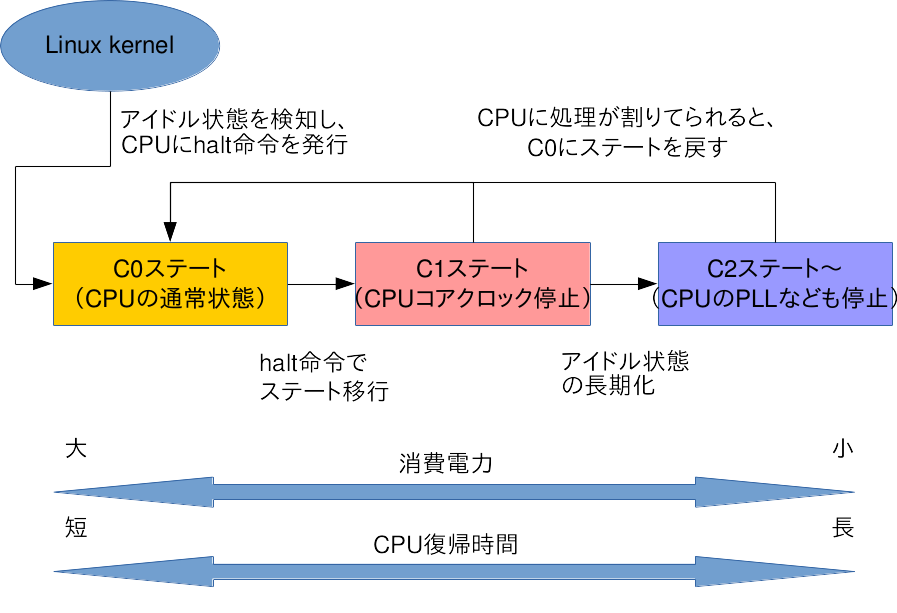
\includegraphics[width=0.8\hsize]{image201602/cpustate.png}
\end{center}
\label{fig:cpustate}
\caption{CPU$B>uBVA+0\4J0W?^(B} 
\end{figure}

\end{frame}

\begin{frame}[containsverbatim]{CPU$B<~GH?t%9%1!<%j%s%05!G=$H(Bcpufreq-info}

Linux $B$N>l9g$O(BCPU$B<~GH?t%9%1!<%j%s%05!G=$,$"$j!"(Bcpufreq $B5!9=$H$7$F(B
$B<BAu$5$l$F$$$k!#(B

\begin{figure}[htbp]
\begin{commandline}
$ cpufreq-info
cpufrequtils 008: cpufreq-info (C) Dominik Brodowski 2004-2009
Report errors and bugs to cpufreq@vger.kernel.org, please.
analyzing CPU 0:
  driver: intel_pstate
  CPUs which run at the same hardware frequency: 0
  CPUs which need to have their frequency coordinated by software: 0
  maximum transition latency: 0.97 ms.
  hardware limits: 800 MHz - 2.90 GHz
  available cpufreq governors: performance, powersave
  current policy: frequency should be within 800 MHz and 2.90 GHz.
                  The governor "powersave" may decide which speed to use
                  within this range.
  current CPU frequency is 1.90 GHz.
....
\end{commandline}
\caption{cpufreq-info $B<B9T7k2L(B}
\label{fig:cpufreq-info}
\end{figure}

\end{frame}

\begin{frame}{$B%,%P%J!<$H8=:_@_Dj$5$l$F$$$k%]%j%7!<(B}

\begin{table}[htb]
\begin{center}
\begin{tabular}{l|l}
$B%,%P%J!<(B & $BFbMF(B \\
ondemand &	CPU$BIi2Y$,Bg$-$$!"$^$?$O>.$5$$;~$K(B \\
         &      CPU$B%/%m%C%/$rBg$-$/$K@Z$jBX$($k(B \\
conservative &	CPU$BIi2Y$,Bg$-$$!"$^$?$O>.$5$$;~$K(B\\
	     &  CPU$B%/%m%C%/$r=y!9$K@Z$jBX$($k(B \\
performance &	$B:GBg<~GH?t$G(BCPU$B$rF0:n$5$;$k(B \\
powersave &	$B:G>.<~GH?t$G(BCPU$B$rF0:n$5$;$k(B \\
userspace &	$B%f!<%6!<$,;XDj$7$?<~GH?t$G(BCPU$B$rF0:n$5$;$k(B \\
\end{tabular}
\caption{$B;XDj$G$-$k%,%P%J!<(B}
\label{tab:governors}
\end{center}
\end{table}

\end{frame}

\begin{frame}[containsverbatim]

\begin{itemize}
\item CPU$B$,(B800MHz$B$+$i(B2.90GHz$B$^$G$r%5%]!<%H$7$F$$$k(B
\item powersave governor $B$GF0:n$7$F$$$k(B
\item $B:GBgCM$H:G>.CM$N%]%j%7!<@_Dj$K$h$j!"(B800MHz$B$+$i(B2.90GHz$B$N4V$GJQF0$5$;$F$$$k(B
\end{itemize}

\begin{commandline}
$ cpufreq-info
cpufrequtils 008: cpufreq-info (C) Dominik Brodowski 2004-2009
Report errors and bugs to cpufreq@vger.kernel.org, please.
analyzing CPU 0:
  driver: intel_pstate
  CPUs which run at the same hardware frequency: 0
  CPUs which need to have their frequency coordinated by software: 0
  maximum transition latency: 0.97 ms.
  hardware limits: 800 MHz - 2.90 GHz
  available cpufreq governors: performance, powersave
  current policy: frequency should be within 800 MHz and 2.90 GHz.
                  The governor "powersave" may decide which speed to use
                  within this range.
  current CPU frequency is 1.90 GHz.
....
\end{commandline}

\end{frame}

\begin{frame}[containsverbatim]{$B%,%P%J!<$H(BCPU$B%/%m%C%/$N@_Dj(B}
$B@_Dj$K$O(B cpufreq-set $B%3%^%s%I$r;H$&!#(B

$B%,%P%J!<$r@_Dj$9$k(B
\begin{commandline}
$ sudo cpufreq-set -c CPU$BHV9f(B -g $B%,%P%J!<L>(B
$B$^$?$O(B
$ sudo sh -c "echo $B%,%P%J!<L>(B > \
  /sys/devices/system/cpu/cpuCPU$BHV9f(B/cpufreq/scaling_governor"
\end{commandline}

\end{frame}

\begin{frame}[containsverbatim]{$B%,%P%J!<$H(BCPU$B%/%m%C%/$N@_Dj(B}

$B:G>.%/%m%C%/$r@_Dj$9$k(B
\begin{commandline}
$ sudo cpufreq-set -c CPU$BHV9f(B -d $B%/%m%C%/CM(B
$B$^$?$O(B
$ sudo sh -c "echo $B%/%m%C%/CM(B > \
  /sys/devices/system/cpu/cpuCPU$BHV9f(B/cpufreq/scaling_min_freq"
\end{commandline}

\end{frame}

\begin{frame}[containsverbatim]{$B%,%P%J!<$H(BCPU$B%/%m%C%/$N@_Dj(B}
$B:GBg%/%m%C%/$r@_Dj$9$k(B
\begin{commandline}
$ sudo cpufreq-set -c CPU$BHV9f(B -u $B%/%m%C%/CM(B
$B$^$?$O(B
$ sudo sh -c "echo $B%/%m%C%/CM(B > \
  /sys/devices/system/cpu/cpuCPU$BHV9f(B/cpufreq/scaling_max_freq"
\end{commandline}

\end{frame}

\begin{frame}[containsverbatim]{$B%,%P%J!<$H(BCPU$B%/%m%C%/$N@_Dj(B}
$B8=:_$N%/%m%C%/$r@_Dj$9$k(B
\begin{commandline}
$ sudo cpufreq-set -c CPU$BHV9f(B -f $B%/%m%C%/CM(B
$B$^$?$O(B
$ sudo sh -c "echo $B%/%m%C%/CM(B > \
  /sys/devices/system/cpu/cpuCPU$BHV9f(B/cpufreq/scaling_cur_freq"
\end{commandline}

\end{frame}

\begin{frame}{$B%,%P%J!<$H(BCPU$B%/%m%C%/$N@_Dj(B}

\begin{itemize}
\item sysfs $B$r;H$C$?@_Dj$O:F5/F0$9$k$H>C$($F$7$^$&!#(B
\item /etc/sysfs.conf $B$r;H$&$+!"(Bcpufreqd $B%Q%C%1!<%8$G@_Dj$G$-$k$h$&$K$9$k!#(B
\end{itemize}

\end{frame}

\begin{frame}{$BF0:n$7$F$$$k%G%P%$%9$N@_Dj(B}

\begin{itemize}
\item $B;H$o$J$$%G%P%$%9$rM-8z$K$9$k$@$1$GEENO$r>CHq$9$k!#(B
\item $B4D6-$K1~$8$F%G%P%$%9$NEENOEy$r@)8f$9$k!#(B
\item $B$3$3$G$O$h$/MxMQ$5$l$k%G%P%$%9$KBP$9$k@)8fJ}K!$K$D$$$F>R2p!#(B
\end{itemize}

\end{frame}

\begin{frame}[containsverbatim]{$B%i%C%W%H%C%W%b!<%I(B}

$B%i%C%W%H%C%W%b!<%I@_Dj(B
\begin{commandline}
$ sudo sh -c "echo 5 > /proc/sys/vm/laptop_mode"
\end{commandline}

NMI watchdog $BL58z2=(B
\begin{commandline}
$ sudo sh -c "echo 0 > /proc/sys/kernel/nmi_watchdog"
\end{commandline}

\end{frame}

\begin{frame}[containsverbatim]{USB}
USB $B$O(B /sys/bus/usb/devices/ $B0J2<$KBP$7$F@_Dj!#(B

\begin{commandline}
$ sudo sh -c "echo off > \
  /sys/bus/usb/devices/usb1/power/control"
$ sudo sh -c "echo auto > \
  /sys/bus/usb/devices/usb1/power/autosuspend"
\end{commandline}

$B5/F0;~$K:F@_Dj$7$?$$>l9g$O(B udev $B$N(B rules $B%U%!%$%k$rMQ0U$9$k!#(B

\begin{commandline}
$ cat /etc/udev/rules.d/70-my-usb-power.rules
ACTION=="add", SUBSYSTEM=="usb", ATTRS{idVendor}=="0x046d", \
      ATTR{idProduct}=="0x08cb", TEST=="power/control", \
      ATTR{power/control}="off"
\end{commandline}

\end{frame}

%$BCm0U$7$J$1$l$P$$$1$J$$E@$H$7$F$O(BUSB$B$r$J$s$G$b@_Dj$7$F$7$^$&$H%-!<%\!<%I$,F0:n$7$J$/$J$k2DG=@-$b$"$k$?$a!"(B
%$B%Y%s%@!<(BID$B!"%G%P%$%9(BID$B$J$I$r3NG'$7$?>e$G@_Dj$7$^$7$g$&!#(B

\begin{frame}[containsverbatim]{$BL5@~(BLAN}

$BL5@~(BLAN$B$O(B iw $B%Q%C%1!<%8$K4^$^$l$k(B iw $B%3%^%s%I$r;H$C$F@_Dj$9$k!#(B

\begin{commandline}
$ sudo iw dev wlan0 set power_save on
\end{commandline}

udev $B$N(B rules $B%U%!%$%k$r;H$C$F@_DjJ}K!(B

\begin{commandline}
$ cat /etc/udev/rules.d/70-my-wifi-power.rules
ACTION=="add", SUBSYSTEM=="net", KERNEL=="wlan*", \
      RUN+="/usr/bin/iw dev %k set power_save on"
\end{commandline}

\end{frame}

\begin{frame}[containsverbatim]{$B%5%&%s%I(B}

\begin{commandline}
$ sudo sh -c "echo 1 > \
  /sys/module/snd_hda_intel/parameters/power_save"
\end{commandline}

\end{frame}

\begin{frame}[containsverbatim]{PCI/PCI-Express}
PCI/PCI-Express $B$N>JEENO$K@_Dj$9$k$K$O(B power/control $B$r(B auto $B$K@_Dj$9$k!#(B

\begin{commandline}
$ sudo sh -c "echo auto > \
  /sys/bus/pci/devices/0000:00:00.0/power/control"
\end{commandline}

\end{frame}

\begin{frame}{$BF0:n$7$F$$$k%W%m%0%i%`$K$D$$$F(B}

\begin{itemize}
\item top $B%3%^%s%I$G$"$kDxEY$o$+$k$,!":Y$+$$?t;z$O$o$+$i$J$$!#(B
\item PowerTOP $B$r;H$C$F3NG'$9$k!#(B
\end{itemize}

\end{frame}

\begin{frame}{$B>JEENO@_Dj$9$k$?$a$N%D!<%k(B}

\begin{itemize}
\item $B>JEENO@_Dj$9$k$K$O@lLg$NCN<1$,I,MW!#(B
\item $B:Y!9$H$7$?@_Dj$r$R$H$D$E$D$d$C$F$$$/$N$OBgJQ!#(B
\item $B@lLgCN<1$,$J$/$F$b!"$6$C$/$j$H$d$C$F$/$l$k%D!<%k$,$"$k!#(B
\item $B$3$l$i$N%D!<%k$r>R2p(B
\end{itemize}

\end{frame}

\begin{frame}{PowerTOP}

\begin{itemize}
\item Intel$B$,3+H/$7$F$$$k%=%U%H%&%'%"!#(B
\item Linux $B%+!<%M%k!"%O!<%I%&%'%"!"%f!<%6%i%s%I$G@)8f2DG=$J>JEENO9`L\$r(B
$BM-8z$K$9$k%D!<%k!#(B
\item $B%W%m%;%9$r4F;k$7$F!"(BCPU$BIi2Y$d%G%P%$%9%I%i%$%P$N;HMQ>u67$N%l%]!<%H$J$I$,9T$($k(B
\end{itemize}

\end{frame}

\begin{frame}[containsverbatim]{$B%$%s%9%H!<%k(B}

\begin{commandline}
% sudo apt-get install powertop	
\end{commandline}

\end{frame}

\begin{frame}[containsverbatim]{$B5/F0(B}

\begin{figure}[H]
\begin{center}
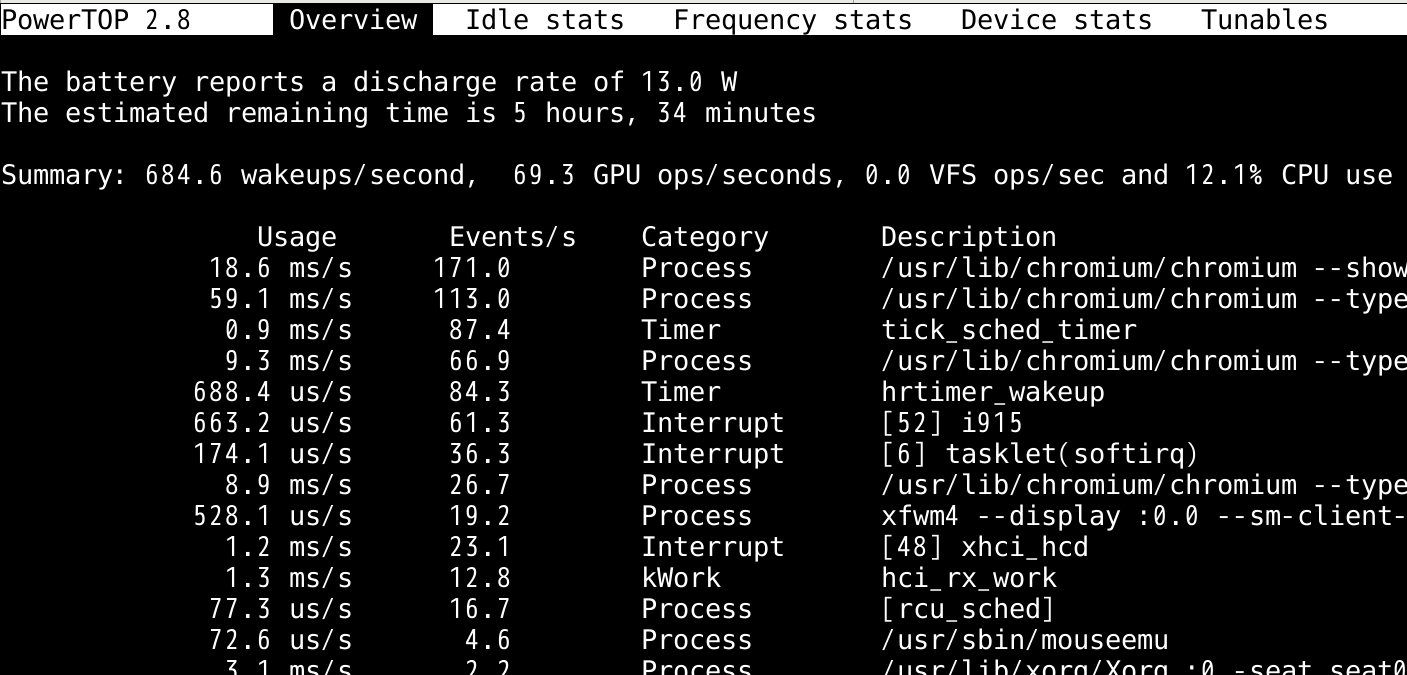
\includegraphics[width=0.8\hsize]{image201602/powertop_00.png}
\end{center}
\label{fig:powertop0}
\caption{PowerTOP$B5/F02hLL(B} 
\end{figure}

\end{frame}

\begin{frame}[containsverbatim]{Tunables $B%?%V(B}
\begin{itemize}
\item Tunables $B%?%V$K$OD4@02DG=$J%7%9%F%`$N@_Dj$,I=<($5$l$k!#(B
\item Bad$B$,>JEENO$KM-8z$J9`L\$K$b$+$+$o$i$:L58z$J@_Dj!#(B
\item Good $B$,4{$KM-8z$K$J$C$F$$$k@_Dj!#(B
\end{itemize}

\begin{figure}[H]
\begin{center}
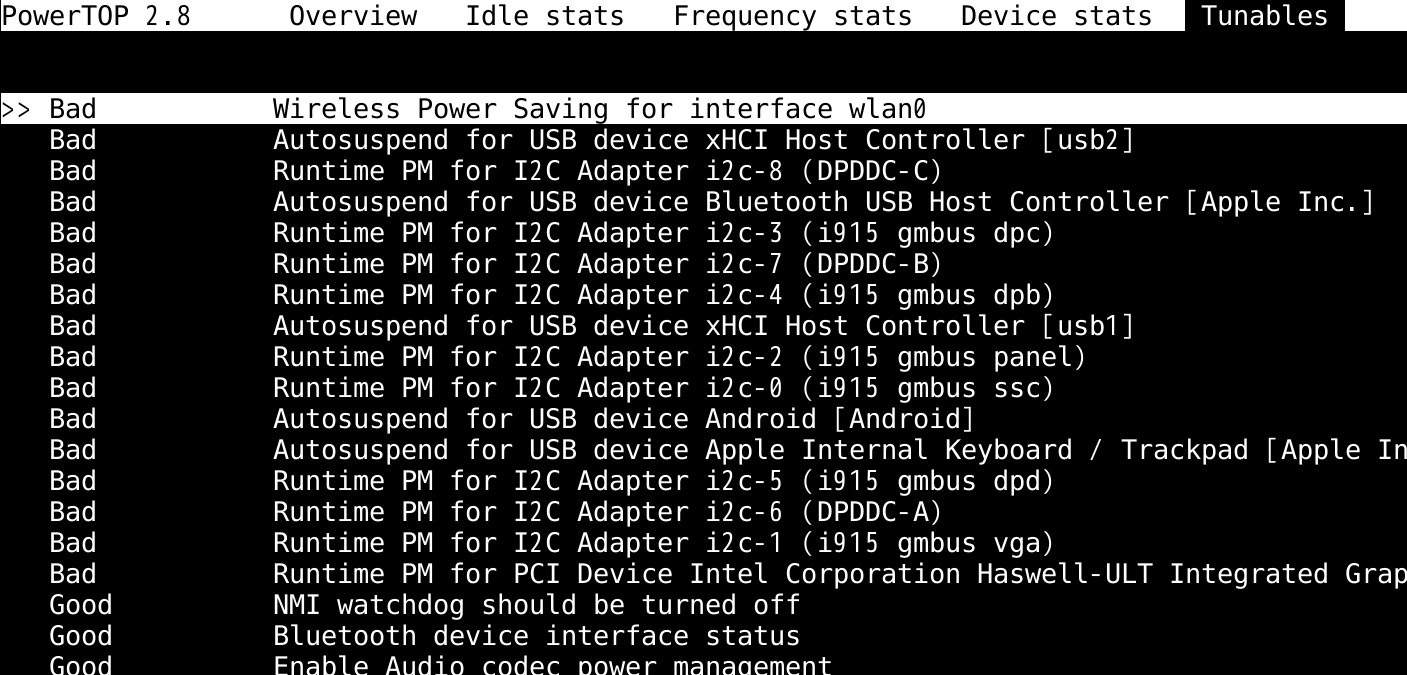
\includegraphics[width=0.8\hsize]{image201602/powertop_01.png}
\end{center}
\label{fig:powertop1}
\caption{Tunables$B2hLL(B} 
\end{figure}

$B$3$N>uBV$G$O$^$@%7%9%F%`$K:GE,2=$5$l$?@_Dj$K$J$C$F$$$J$$$?$a!"0lEY=*N;$7!"(B
$B%-%c%j%V%l!<%7%g%s$r9T$&!#(B

\end{frame}

\begin{frame}[containsverbatim]{$B%-%c%j%V%l!<%7%g%s(B}

$B<B9T$9$k$H%G%P%$%9$J$I$+$i;HMQ>u67$rFI$_<h$j!"%^%7%s$KBP$7$FE,@Z$J@_Dj$r(B
$B9T$&!#(B
$B%N!<%H(BPC$B$N>l9g$O$$$-$J$j%b%K%?!<$N%P%C%/%i%$%H$,>C$($k$N$GCm0U!#(B

\begin{commandline}
$ sudo powertop --calibrate
\end{commandline}

\end{frame}

\begin{frame}[containsverbatim]{$B%-%c%j%V%l!<%7%g%s(B}

\begin{itemize}
\item $B%-%c%j%V%l!<%7%g%s$,=*$o$k$H!"(B\texttt{/var/cache/powertop/saved\_parameters.powertop}
$B0J2<$K%G!<%?$,J]B8$5$l$k!#(B
\item $B<!2s$N(BPowerTOP$B5/F0;~$+$i$O%-%c%j%V%l!<%7%g%s%G!<%?$r85$K(B
$B>JEENO$K$5$l$?4D6-$G5/F0$9$k!#(B
\end{itemize}

\end{frame}

\begin{frame}[containsverbatim]{$B%-%c%j%V%l!<%7%g%s8e(B}

$B%-%c%j%V%l!<%7%g%s8e$K5/F0$9$k$H!"(B
$B!V(BThe battery reports a discharge rate ...$B!W(B $B$N9`L\$KI=<($5$l$k>CHqEENOCM$,JQ$o$j!"%7%9%F%`(B
$BA4BN$G>JEENO$G2TF/$7$F$$$k;v$,3NG'$G$-$k$O$:!#(B

\end{frame}

\begin{frame}[containsverbatim]{PowerTOP $B$N5/F0;~M-8z2=(B}

\begin{itemize}
\item PowerTOP $B$O5/F0$9$k$HJ]B8$5$l$F$$$k@_Dj$r85$K>JEENO>uBV$K$7$F$/$l$^$9$,!"(BPC$B$rN)$A>e$2$k$?$S$K(B
PowerTOP$B<+BN$rN)$A>e$2$kI,MW$,$"$k!#(B
$B!#(B

\item $B5/F0;~$K<+F0E*$K(BPowerTOP $B$rN)$A>e$2$k$h$&$K$9$k$K$O!"0J2<$N$h$&$K(B systemd $B$N(B $B%f%K%C%H%U%!%$%k(B
$B$rMQ0U$7!"M-8z$K$9$k!#(B

\begin{commandline}
$ cat /etc/systemd/system/powertop.service

[Unit]
Description=PowerTOP

[Service]
Type=oneshot
ExecStart=/usr/bin/powertop
Environment="TERM=xterm"

[Install]
WantedBy=multi-user.target
\end{commandline}

\begin{commandline}
$ sudo systemctl enable powertop
\end{commandline}

\end{itemize}

\end{frame}

\begin{frame}[containsverbatim]{TLP $B$r;H$C$?@_Dj(B}

\begin{itemize}
\item PowerTOP$B$N$h$&$K>\:Y$J%l%]!<%H$O(B
$B=P$5$J$$$,!"(BAC$B@\B3;~$J$I$N>u67$K1~$8$?%9%/%j%W%H$,=`Hw$5$l$F$*$j!"%$%s%9%H!<%k(B
$B$9$k$@$1$G$"$kDxEY>JEENO@_Dj$r9T$C$F$/$l$kJXMx$J%D!<%k!#(B
\item Debian $B$G$O%Q%C%1!<%82=$5$l$F$*$j!"(Bapt $B$G%$%s%9%H!<%k$G$-$k!#(B
\begin{commandline}
$ sudo apt-get install tlp
\end{commandline}

\end{itemize}

\end{frame}


\begin{frame}[containsverbatim]{TLP $B$r;H$C$?@_Dj(B}

\begin{itemize}
\item $BL5@~(BLAN$B$N@_DjEy$K(B NetworkManager $B$r;H$C$F$$$k$J$i(B tlp-rdw $B%Q%C%1!<%8$b%$%s%9%H!<%k$7$F$*$/$H(B
$BL5@~(BLAN$B!"(BBluetooth$B4XO"$N@_Dj$b9T$C$F$/$l$k!#(B

\item $B%G%U%)%k%H$N@_Dj$O(B /etc/default/tlp $B$K$"$j!"$3$N%U%!%$%k$rJQ99$7$F4D6-$K9g$o$;$?>JEENO@_Dj$r(B
$B9T$&!#(B

\end{itemize}
\end{frame}

\begin{frame}[containsverbatim]{TLP $B$r;H$C$?@_Dj(B}
\begin{itemize}

\item $B@_Dj$O$h$/;H$o$l$k9`L\$7$+$J$/!";H$C$F$$$k4D6-$N@_Dj$,$J$$>l9g$b$"$k!#$3$N$h$&$J>l9g$O(B
$B<+J,$G@_Dj$rDI2C$9$k$+!"@h$K@bL@$7$?$h$&$K(Bsysfs / procfs $B7PM3(B
$B$N@_Dj$rJLES9T$&I,MW$,$"$k!#(B

\begin{center}
\begin{commandline}
# Set to 0 to disable, 1 to enable TLP.
TLP_ENABLE=1

# Operation mode when no power supply can be detected: AC, BAT
# Concerns some desktop and embedded hardware only.
TLP_DEFAULT_MODE=AC

# Seconds laptop mode has to wait after the disk goes idle before doing a sync.
# Non-zero value enables, zero disables laptop mode.
DISK_IDLE_SECS_ON_AC=0
DISK_IDLE_SECS_ON_BAT=2

# Dirty page values (timeouts in secs).
MAX_LOST_WORK_SECS_ON_AC=15
MAX_LOST_WORK_SECS_ON_BAT=60
...
\end{commandline}
\end{center}

TLP $B$O(B systemd $B$d$=$NB>(Binit$BMQ$N5/F0%U%!%$%k$,MQ0U$5$l$F$$$k$N$G(BPC$B5/F0;~$K@_Dj$,H?1G$5$l$k$N$b(B
$BNI$$E@$G$9!#(B

\end{itemize}

\end{frame}

\begin{frame}{$B>JEENO@_Dj8e(B}
\begin{itemize}
\item $B>JEENO@_Dj$7$?8e$K(B PowerTOP $B$G>CHqEENO$r3NG'!#(B
\item $B>CHqEENO$,(B13W $B$+$i(B 11W $B$K2<$,$C$F$$$k!#(B
\item PC$B2TF/;~4V$b(B5$B;~4VH>$+$i(B6$B;~4V(B50$BJ,$K?-$S$F$$$k(B
\end{itemize}

\begin{figure}[H]
\begin{center}
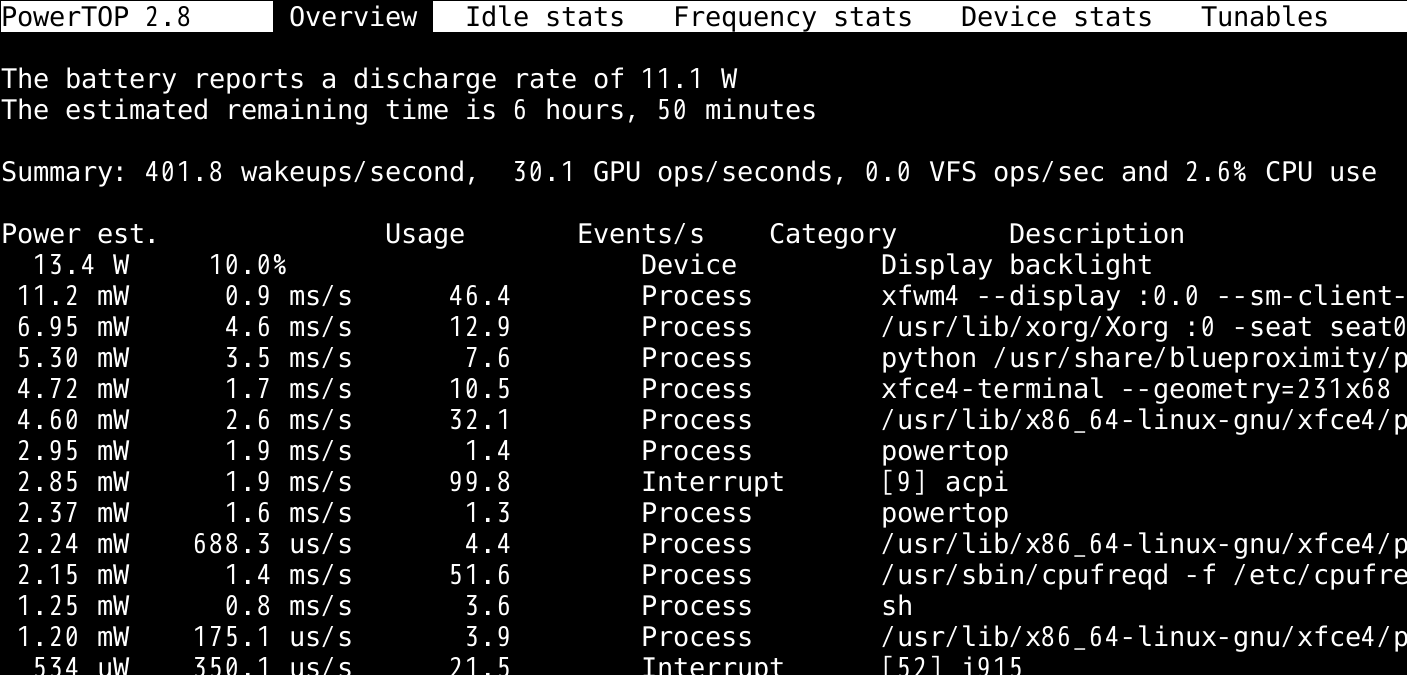
\includegraphics[width=0.8\hsize]{image201602/powertop_02.png}
\end{center}
\label{fig:powertop2}
\caption{$B>JEENO@_Dj8e(B} 
\end{figure}

\end{frame}

\begin{frame}{$B$^$H$a(B}

\begin{itemize}

\item Debian GNU/Linux$B$G$N>JEENO@_Dj$K$D$$$F@bL@$7$?!#(B
\item $B8=:_$N>uBV$r$H$j$"$($:3NG'$9$k$K$O(B cpufreq-info $B$r;H$$!"%+!<%M%k$N@_Dj$d%I%i%$%P$N@_Dj$O(B
sysfs $B$d(B proc fs $B7PM3$G@_Dj$9$k!#(B
\item $B%W%m%0%i%`$d%W%m%;%9$N>\:Y$J>uBV$N3NG'$9$k$K$O(B
PowerTOP$B$r;H$&!#>JEENO@_Dj$G$-$k9`L\$b$o$+$j!"%f!<%6%$%s%?!<%U%'%$%9$+$i3F<o@_Dj$,$G$-$k$h$&$K$J$C$F$$$k!#(B
%\item PC$B$r:FN)$A>e$2$9$k$H(B PowerTOP $B$r5/F0$5$;$kI,MW$,$"$k$?!"(Bsysytem$BMQ$N(Bservice$B%U%!%$%k$rJLESMQ0U$9$k$J$I$NBP:v$,I,MW$G$9!#(B
\item
$B:Y$+$$@_Dj$r9T$o$J$/$F$b!"$H$j$"$($:>JEENO@_Dj$r9T$$$?$$>l9g$O(BTLP$B$r;H$&$N$,$h$$!#$?$@A4$F$N(BPC$B$r%5%]!<%H$7$F$$$k$o$1$G$O$J$$$N$G!"4D6-$K9g$o$;$F%W%m%0%i%`$r=$@5$9$k$J$j$NBP1~$,I,MW$H$J$k!#(B
\item $B:Y$+$$@_Dj$r$7$?$$>l9g$O(B sysfs $B$d(B procfs$B$+$i@_Dj$9$kI,MW$,$"$k!#$3$N>l9g@lLg$NCN<1$,I,MW$H$J$k!#(B

\end{itemize}
\end{frame}


\section{libhinawa $B$H$$$&%i%$%V%i%j$r(B Debian $B%W%m%8%'%/%H$K(B ITP/RFS $B$7$?OC(B}
\emtext{libhinawa $B$H$$$&%i%$%V%i%j$r(B Debian $B%W%m%8%'%/%H$K(B ITP/RFS $B$7$?OC(B}

\begin{frame}{$B35MW(B}
  libhinawa$B$H$$$&%i%$%V%i%j$r(BDebian$B%W%m%8%'%/%H$K(BITP/RFS$B$7$?$N$G!"(B
  $B$=$NGX7J$d@_7W!"5!G=$K4X$7$F!"(BALSA$B$N(Bupstream$B$G$N3hF0$bF'$^$($F(B
  $B$*OC$7$^$9!#(B
\end{frame}

\begin{frame}{$BFbMF(B}
  \begin{itemize}
  \item ALSA$B$K$D$$$F(B
  \item libhinawa$B$K$D$$$F(B
  \item $B:#2s$N(BITP/RFS$B$K$D$$$F(B
  \end{itemize}
  $B<A5?$OE,599T$C$F$/$@$5$$!#(B
\end{frame}

\begin{frame}{ALSA$B$N35MW(B}
  ALSA
  \begin{itemize}
  \item Linux sound subsystem
  \item $B%f!<%6!<%9%Z!<%9$N%"%W%j%1!<%7%g%s$KBP$7!"%5%&%s%I%G%P%$%9$r(B
        $B@)8f$9$k<jCJ$rDs6!(B
  \item $BFCDj$N%5%&%s%I%G%P%$%9$KBP$7$F$O!"(BCUI$B$d(BGUI$B$rH<$&%D!<%k$rDs6!(B
  \end{itemize}
  ALSA$B$rMxMQ$7$F$$$k$b$N(B
  \begin{itemize}
  \item Linux$B%+!<%M%k$r:NMQ$7$?@=IJA4HL(B
  \end{itemize}
\end{frame}

\begin{frame}{ALSA$B$,%5%]!<%H$9$k%5%&%s%I%G%P%$%9(B}
  \begin{itemize}
  \item PCI/PCI-Express$B%P%9$K@\B3$9$k$b$N(B
  \item $B%W%i%C%H%U%)!<%`8GM-$N%Z%j%U%'%i%k%P%9$K@\B3$9$k$b$N(B
  \item USB$B$K@\B3$9$k$b$N(B
  \item $BB>!"%l%,%7!<$JHFMQ%P%9$K@\B3$9$k$b$N(B (IEEE 1394$B%P%9(B)
  \end{itemize}
\end{frame}

\begin{frame}{ALSA$B$H(BIEEE 1394$B%P%9(B}
  2000-2010$BG/$K$+$1$F!"(BIEEE 1394$B%P%9$K@\B3$7$F;H$&(B
  $B%5%&%s%I%G%P%$%9$,H/Gd$5$l$F$$$?!#(B
  \begin{itemize}
  \item $B<g$K%l%3!<%G%#%s%0MQES(B
  \item $B0lIt$N9b5i%*!<%G%#%*5!4o(B
  \end{itemize}
  ALSA$B$G$N%5%]!<%H$O(B2010$BG/$K;O$^$C$?!#(B
  \begin{itemize}
  \item Linux 2.6.39$B$K=i4|$N%3!<%I$r%^!<%8(B
  \item $B0J9_$N3+H/$O?J$^$:(B
  \end{itemize}
\end{frame}

\begin{frame}{$B%f!<%6!<%9%Z!<%9$N%I%i%$%P<BAu(B}
  Linux FireWire subsystem$B$,!"%-%c%i%/%?%G%P%$%91[$7$K(B
  $B%G%P%$%9$r@)8f$9$k<jCJ$r%f!<%6!<%9%Z!<%9$KDs6!(B
  \begin{itemize}
  \item /dev/fw[0-9]*
  \end{itemize}
  FFADO
  \begin{itemize}
  \item $B%f!<%6!<%9%Z!<%9$N%I%i%$%P3+H/%W%m%8%'%/%H(B
  \item \url{http://ffado.org/}
  \item libffado2$B$H$7$F!"(BC$B$N%i%$%V%i%j(BAPI$B$r8x3+(B
  \item 2004$BG/$"$?$j$K3+H/3+;O(B
  \end{itemize}
  ALSA$B$H$O0[$J$k(BAPI
  \begin{itemize}
  \item ALSA$B$N%"%W%j%1!<%7%g%s$+$i;H$($J$$(B
  \item $B%W%m%H%3%k;EMM(B(IEC 61883-1/6)$BE*$K!"(BALSA-FFADO
        $B%V%j%C%8$,@.N)$7$J$$!#(B
  \end{itemize}
\end{frame}

\begin{frame}{ALSA$B$N(Bfirewire$B%9%?%C%/$N@.D9(B}
  2013$BG/(B1$B7n;~E@!#(B2$B%b%G%k$r%5%]!<%H!#(B
  \begin{itemize}
  \item 2,600$B9TDxEY(B
  \end{itemize}
  2016$BG/(B2$B7n8=:_!"Ls(B140$B%b%G%k$r%5%]!<%H$9$k$K;j$k!#(B
  \begin{itemize}
  \item 20,000$B9TDxEY(B
  \end{itemize}
\end{frame}

\begin{frame}{libhinawa$B$N35MW(B}
  ALSA$B$N(Bfirewire$B%9%?%C%/$N@_7W(B
  \begin{itemize}
  \item $B%j%"%k%?%$%`%G!<%?E>Aw0J30$N5!G=$O%f!<%6!<%9%Z!<%9$KCV$/(B
  \item $B$I$&$7$F$b%+!<%M%k%i%s%I$KI,MW$J5!G=$O(BALSA$B$N(BHwDep$B$r;H$C$F(B
        $B%f!<%6!<%9%Z!<%9$+$i%"%/%;%92DG=$K$9$k(B
  \end{itemize}
  $BEv=i$O(BFFADO$B$N;q;:$r:FMxMQ$9$k$D$b$j$@$C$?(B
  \begin{itemize}
  \item $B$,!"$=$l$O:$Fq$rH<$&$3$H$,8e$KH=L@(B
  \end{itemize}
\end{frame}

\begin{frame}{FFADO$B$N:$Fq(B}
  FFADO$B$N%D!<%k$r3+H/$KMQN)$F$k$N$O$`$D$+$7$$(B
  \begin{itemize}
  \item libffado2$B$N@_7W>e$N7g4Y(B
  \end{itemize}
  FFADO$B$N%3!<%I%Y!<%9$N8E$5(B
  \begin{itemize}
  \item FFADO$B$N%D!<%k$,(BPython2$B$G=q$+$l$F$$$k(B
  \end{itemize}
  $B3+H/$KMQN)$F$k%D!<%k$NI,MW(B
  \begin{itemize}
  \item libhinawa$B$N3+H/$KCe<j(B
  \end{itemize}
\end{frame}

\begin{frame}{libhinawa$B$N@_7W(B}
  $B%-%c%i%/%?%G%P%$%9$KBP$9$kF~=PNO$NCj>](B
  \begin{itemize}
  \item /dev/fw[0-9]*
  \item /dev/snd/hwC[0-9]*D0
  \end{itemize}
  GObject Introspection$B$K$h$k!"8@8l%P%$%s%G%#%s%0$+$i$NMxMQ(B
  \begin{itemize}
  \item 140$B%G%P%$%9$=$l$>$l8GM-$NA`:n$,I,MW(B
  \item $B%G%P%$%9A`:nJ}K!$r8+=P$9;n9T:x8m$,I,MW(B
  \item LL$B$G=q$-$?$+$C$?(B
  \end{itemize}
\end{frame}

\begin{frame}{libhinawa$B$N3+H/(B}
  \begin{itemize}
  \item 2014$BG/(B9$B7n$"$?$j$K3+H/Ce<j!#(BC$B$N%i%$%V%i%j(BAPI$B$r8x3+(B (0.2.0)
  % [alsa-devel] [RFC] libhinawa: a light-weight I/O library for
status/transactions to ALSA FireWire devices
  %
\url{http://mailman.alsa-project.org/pipermail/alsa-devel/2014-September/081732.html}
  \item 2015$BG/(B1$B7n$K(BGObject Introspection$BBP1~(B (0.3.0)
  % [alsa-devel] [RFC] libhinawa: gobject introspection library for
ALSA/FireWire transaction
  %
\url{http://mailman.alsa-project.org/pipermail/alsa-devel/2015-January/086371.html}
  \item $B$=$N(B2$B=54V8e$K(Balsa-tools.git$B$KBP$9$k(BRFC (0.4.0)
  % [alsa-devel] [RFC][PATCH 00/13] alsa-tools: libhinawa for control
applications of FireWire devices
  %
\url{http://mailman.alsa-project.org/pipermail/alsa-devel/2015-January/086969.html}
  \item 2015$BG/(B2$B7n$K(Balsa-lib$B$X$N0MB8$rGK4~(B (0.5.0)
  \end{itemize}
\end{frame}

\begin{frame}{libhinawa$B$N3+H/(B($B$D$E$-(B)}
  \begin{itemize}
  \item 2015$BG/(B3$B7n$K=i4|$N(Bdebian/rpm$B%Q%C%1!<%8%s%0$H$=$l$KH<$&=$@5(B (0.6.0)
  \item 2016$BG/(B1$B7n$K(BDebian$B$X$N(BITP$B$H$=$l$KH<$&=$@5(B (0.7.0)
  %[alsa-devel] About planning of libhinawa ITP to debian project
  %
\url{http://mailman.alsa-project.org/pipermail/alsa-devel/2016-February/103771.html}
  \end{itemize}
\end{frame}

\begin{frame}{libhinawa$B3+H/$NN"(B}
  $B%a%$%s%i%$%s$N:n6H(B
  \begin{itemize}
  \item Linux 3.16 - 63$B%Q%C%A(B
  %\item https://lkml.org/lkml/2014/6/4/895
  \item Linux 3.19 - 31$B%Q%C%A(B
  %\item https://lkml.org/lkml/2014/12/11/226
  \item Linux 4.2 - 22$B%Q%C%A(B
  %\item https://lkml.org/lkml/2015/6/25/59
  \item Linux 4.4 - 68$B%Q%C%A(B
  %\item https://lkml.org/lkml/2015/11/6/410
  \end{itemize}
  Linux stable kernel
  \begin{itemize}
  \item $B%P%0$,Js9p$5$l$?$i!"$=$N=$@5%Q%C%A$r:n$C$F(Bstable$B$KAw$k!#(B
  \end{itemize}
\end{frame}

\begin{frame}{libhinawa$B$N(BITP/RFS}
  $B:n6H$O(Bgithub$B$r;H$C$F?J$a$k!#(B
  \begin{itemize}
  \item \url{https://github.com/takaswie/libhinawa/}
  \end{itemize}
  1/14$B$"$?$j(B
  \begin{itemize}
  \item $BNS$5$s$H!"(Blibhinawa$B$N(BITP$B$NOC$r$9$k!#(B
  \end{itemize}
  1/18
  \begin{itemize}
  \item $BNS$5$s$+$i:G=i$N(BPR
  \end{itemize}
  1/24$B$"$?$j(B
  \begin{itemize}
  \item Ubuntu 16.04$B$N(BDebianImportFreeze(2/17)$B$K4V$K9g$o$;$kJ}?K(B
  % https://wiki.ubuntu.com/XenialXerus/ReleaseSchedule
  \end{itemize}
  1/28$B$"$?$j(B
  \begin{itemize}
  \item Autotools$B<~$j$N=$@5=*N;(B
  \item debian/* $B$NMQ0U=*N;(B
  \end{itemize}
\end{frame}
\begin{frame}{libhinawa$B$N(BITP/RFS($B$D$E$-(B)}
  1/31
  \begin{itemize}
  \item Debian$B%W%m%8%'%/%H$K(BITP$B$9$k$3$H$r!"(BLinux FireWire subsystem,
        Linux sound subsystem$B!"(BFFADO$B$KBP$7$FO"Mm!#(B
  \item
\url{http://mailman.alsa-project.org/pipermail/alsa-devel/2016-January/103693.html}
  \end{itemize}
  2/2
  \begin{itemize}
  \item ITP
  \begin{itemize}
  \item \url{https://bugs.debian.org/cgi-bin/bugreport.cgi?bug=813474}
  \end{itemize}
  \item RFS
  \begin{itemize}
  \item \url{https://bugs.debian.org/cgi-bin/bugreport.cgi?bug=813489}
  \end{itemize}
  \end{itemize}
\end{frame}

\begin{frame}{Debian$B$X$N(BITP/RFS$B8e(B}
  2/6
  \begin{itemize}
  \item $BHu8}BgJe$5$s$K%9%]%s%5!<%I$7$F$b$i$&(B
  \item New queue$BF~$j$9$k(B
  \end{itemize}
  2/7
  \begin{itemize}
  \item $BD+!"(Bftp-master$BF~$j!#(Bunstable$B%j%]%8%H%j$KF~$k(B
  \begin{itemize}
  \item \url{https://packages.debian.org/source/sid/libhinawa}
  \end{itemize}
  \item $BLk!"(BUbuntu$B$N(BDebian AutoSync bot$B$,JaB*!#(Buniverse$B%j%]%8%H%j$KF~$k!#(B
  \begin{itemize}
  \item \url{https://launchpad.net/ubuntu/+source/libhinawa}
  \end{itemize}
  \item $B?<Lk!"%"%C%W%9%H%j!<%`$KJs9p(B
  \begin{itemize}
  \item
\url{http://mailman.alsa-project.org/pipermail/alsa-devel/2016-February/104046.html}
  \end{itemize}
  \end{itemize}
\end{frame}

\begin{frame}{$B$^$H$a(B}
\begin{itemize}
\item libhinawa$B$r(BDebian$B%W%m%8%'%/%H$K(BITP$B$7$^$7$?(B
\end{itemize}
\end{frame}

\section{Hack time}
\emtext{Hack time}

\begin{frame}{$B@.2L$r5-F~2<$5$$(B!}

  $B:#2s!"(BHack time$B;~$N@.2L$r5-O?$K;D$7$F$_$^$9!#(B

\url{https://debianmeeting.titanpad.com/8}

$B$K3'$5$s%"%/%;%9D:$-!JG'>ZITMW$G$9!K!"3F<+@.2L$r(B18:40$B$^$G$K5-O?$9$k$h$&$K$*$M$,$$$7$^$9!#(B

\end{frame}
  
\section{$B:#8e$N%$%Y%s%H(B}
\emtext{$B:#8e$N%$%Y%s%H(B}
\begin{frame}{$B:#8e$N%$%Y%s%H(B}
\begin{itemize}
\item 2/16 Debian developer$BMhF|7^7b(BGPG Beer Signing(2016/2)
 Debian$B$K$F!"(BLXDE$B$N%Q%C%1!<%8%a%s%F%J$r$5$l$F$$$k(BAndrew Lee$B$5$s$,MhF|$5$l!"(Bhenrich$B$5$s$K$F!"0{$_2q$7$J$,$i$N%-!<%5%$%s2q$,9T$o$l$^$9!#7G<(!'(B\url{http://debianjp.connpass.com/event/26965/}
\item $B4X@>%(%j%"(BDebian$BJY6/2q!#(B
\end{itemize}
\end{frame}

\begin{frame}{$B:#8e$N%$%Y%s%H(B}
\begin{itemize}
\item 3/5 ($BEZ(B) $BBh(B137$B2sEl5~%(%j%"(BDebian$BJY6/2q(B\\
  $B>l=j$O%5%$%\%&%:3t<02q<R$5$s$K$F!*$3$NF|!"(Bhenrich$B$5$s$N$*<jG[$K$h$j!"%I%$%D$+$i8x<0(BDebian Developer$B$N(BJohn Paul Adrian Glaubitz$B$5$s$,9gN.$5$l$^$9!*3$30(B Developer$B$N(BKey Sign$B$N%A%c%s%9!"3$30$N%"%/%F%#%V$J(BDebian Developer$B$NJ}$H$V$C$A$c$1%H!<%/$J$I=PMh$k5.=E$J%A%c%s%9!*$5$"!"$=$3$N5.J}$b;22C$9$k$N$@!#(B
\end{itemize}
\end{frame}

\begin{frame}{$B:#8e$N%$%Y%s%H!J$D$E$-!K(B}
\begin{itemize}
\item $B;29M!'(BAndrew Lee$B$5$s$N3hF0(B\\
   \url{https://qa.debian.org/developer.php?login=ajqlee}\\
    $B<g$K(BLXDE $B%G%9%/%H%C%W4D6-$N%Q%C%1!<%8$J$I!#(B
\item $B;29M!'(BJohn Paul Adrian Glaubitz$B$5$s$N3hF0(B
  \begin{itemize}
  \item $B>\$7$/$O!"(B\url{https://qa.debian.org/developer.php?login=glaubitz\%40physik.fu-berlin.de} Debian$B$N(BMATE $B%G%9%/%H%C%W4D6-$NB??t$N%Q%C%1!<%872$J$I!#(B
  \item m68k/sh4/sparc64$B0\?":n6H(B
  \end{itemize}
\end{itemize}
\end{frame}

\section{$B:#F|$N1c2q>l=j(B}
\emtext{$B:#F|$N1c2q>l=j(B}
\begin{frame}{$B:#F|$N1c2q>l=j(B}
$BL$Dj(B
\end{frame}

\end{document}

;;; Local Variables: ***
;;; outline-regexp: "\\([ 	]*\\\\\\(documentstyle\\|documentclass\\|emtext\\|section\\|begin{frame}\\)\\*?[ 	]*[[{]\\|[]+\\)" ***
;;; End: ***
